\documentclass[24pt,pdf,hyperref={unicode}]{beamer}
\usepackage[utf8]{inputenc}
\usepackage{aiml}

\begin{document}

\newcommand{\myrect}[5] 
{
\draw[thick] (#1,#2) rectangle ($(#1+#3,#2+#4)$); 
\node at ($(#1,#2)+(#3 /2,#4 /2)$) {#5};
}
\usetikzlibrary{calc}

\begin{frame}
\begin{columns}
\column{0.5\textwidth}

\uncover<1->{
\begin{tikzpicture}[x=0.7cm, y=0.7cm]
\myrect{0}{0}{6.5}{1}{Table}
\myrect{0.5}{1}{1}{1}{A}
\myrect{2}{1}{1.5}{1.5}{B}
\myrect{4}{1}{2}{2}{C}
\end{tikzpicture}
}

{\small
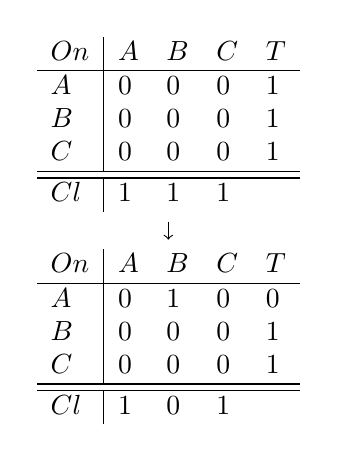
\begin{tikzpicture}[x=1cm,y=-2.7cm]
\uncover<3->{
\node(a+b+c) at (0,0) {$
\begin{array}{l|l l l l}
On & A & B & C & T \\
\hline
A  & 0 & 0 & 0 & 1 \\
B  & 0 & 0 & 0 & 1 \\
C  & 0 & 0 & 0 & 1 \\
\hline\hline 
Cl & 1 & 1 & 1 & \\
\end{array}$};
}

\uncover<4->{
\node(ab+c) at (0,1) {$
\begin{array}{l|l l l l}
On & A & B & C & T \\
\hline
A  & 0 & 1 & 0 & 0 \\
B  & 0 & 0 & 0 & 1 \\
C  & 0 & 0 & 0 & 1 \\
\hline\hline 
Cl & 1 & 0 & 1 & \\
\end{array}$};

\path (a+b+c) edge[->] (ab+c);
}


\end{tikzpicture}
}


\column{0.5\textwidth}

\uncover<2->{
Действие:

\begin{itemize}
\item $ Move(what,from,to)$
\end{itemize}

Требования:


\begin{itemize}
\item $On(what,from)$
\item $Cl(to) \vee (to=Table)$
\item $Cl(what)$
\end{itemize}

Результат:

\begin{itemize}
\item $On(what,to)$
\item $\neg Cl(to)$
\item $\neg On(what,from)$
\item $Cl(from)$
\end{itemize}
}

\end{columns}
\end{frame}

\begin{frame}
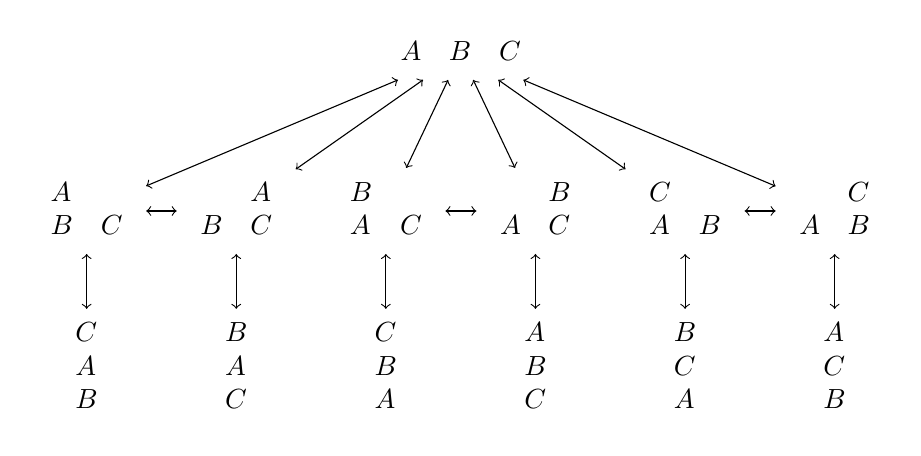
\begin{tikzpicture}[x=1.9cm, y=-2cm]

\uncover<1->{
\node (a+b+c) at (2.5,0) {$\begin{array}{l l l} A & B & C \end{array}$};
}

\uncover<2->{
\node(ab+c) at (0,1) {$\begin{array}{l l} A \\ B & C \end{array}$};
\path (a+b+c) edge[<->] (ab+c);
}

\uncover<3->{
\node(ac+b) at (1,1) {$\begin{array}{l l} & A \\ B & C \end{array}$};
\node(ba+c) at (2,1) {$\begin{array}{l l} B \\ A & C \end{array}$};
\node(bc+a) at (3,1) {$\begin{array}{l l} & B \\ A & C \end{array}$};
\node(ca+b) at (4,1) {$\begin{array}{l l} C \\ A & B \end{array}$};
\node(cb+a) at (5,1) {$\begin{array}{l l} & C \\ A & B \end{array}$};

\path (a+b+c) edge[<->] (ac+b);
\path (a+b+c) edge[<->] (ba+c);
\path (a+b+c) edge[<->] (bc+a);
\path (a+b+c) edge[<->] (ca+b);
\path (a+b+c) edge[<->] (cb+a);
}

\uncover<4->{
\path (ab+c) edge[<->] (ac+b);
\path (ba+c) edge[<->] (bc+a);
\path (ca+b) edge[<->] (cb+a);
}

\uncover<5->{
\node(cab) at (0,2) {$\begin{array}{l} C \\ A \\ B \end{array}$};
\node(bac) at (1,2) {$\begin{array}{l} B \\ A \\ C \end{array}$};
\node(cba) at (2,2) {$\begin{array}{l} C \\ B \\ A \end{array}$};
\node(abc) at (3,2) {$\begin{array}{l} A \\ B \\ C \end{array}$};
\node(bca) at (4,2) {$\begin{array}{l} B \\ C \\ A \end{array}$};
\node(acb) at (5,2) {$\begin{array}{l} A \\ C \\ B \end{array}$};

\path (ab+c) edge[<->] (cab);
\path (ac+b) edge[<->] (bac);
\path (ba+c) edge[<->] (cba);
\path (bc+a) edge[<->] (abc);
\path (ca+b) edge[<->] (bca);
\path (cb+a) edge[<->] (acb);
}

\end{tikzpicture}
\end{frame}

\begin{frame}
\begin{center}
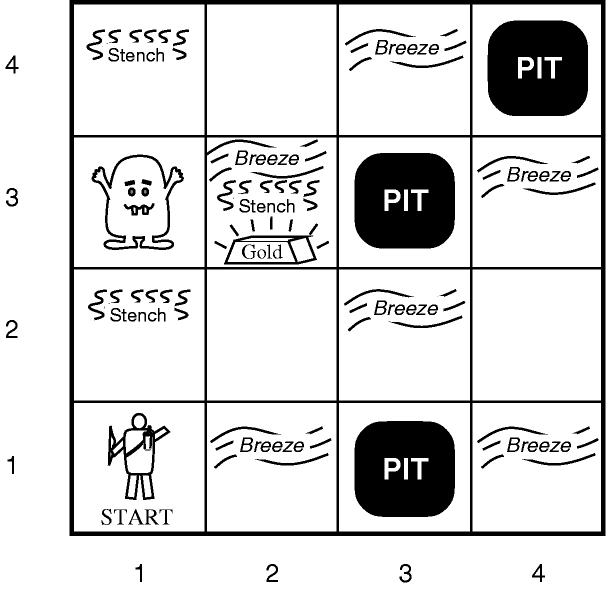
\includegraphics[width=0.7\textwidth]{wumpus.png}
\end{center}
\end{frame}



\end{document}
